% !TEX root = ../BeamerTemplate.tex
%%%%%%%%%%%%%%%%%%%%%%%%%%%%%%%%%%%%%%%%%%%%%%%%%%%%%%%%%%%%%%%%%%%%%%%%%%%%%%%%%%

\section{New commands}
\begin{frame}[fragile]{New commands}
The various commands presented in my other templates (book, article) compatible with Beamer can be used. A list of these commands is provided in those other templates, which can be found at the following link:

\vspace{.5cm}\url{https://mattiapuddu25.github.io/index.html}
\end{frame}

\section{PGF and Tikzpicture}

\begin{frame}[fragile]{PGF and Tikzpicture}{PGF and Tikzpicture}
As with commands, graphs can also be created in Beamer using pgfplots and TikZ. Here I present some examples (different from those I included in the book and Beamer templates):
\end{frame}

\begin{frame}[fragile]{PGF and Tikzpicture (second part)}{PGF and Tikzpicture (second part)}
\begin{figure}[ht]
\centering
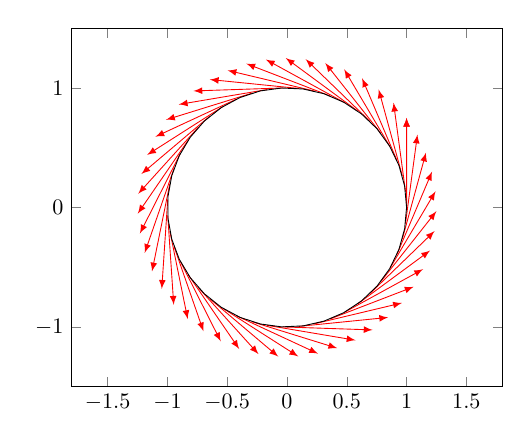
\begin{tikzpicture}[scale=.8]
    \begin{axis}[xmin=-1.5, xmax=1.5, ymin=-1.5, ymax=1.5, axis equal]
    
        \addplot[samples=48, domain=0:2*pi, -latex, variable=\t,
            quiver={u={-sin(deg(t))},
                    v={cos(deg(t))},
                    scale arrows=0.75,
                    colored=red}]
                ({cos(deg(t))}, {sin(deg(t))});
       
        \addplot[samples=36, domain=0:2*pi]
            ({cos(deg(x))}, {sin(deg(x))});
    \end{axis}
\end{tikzpicture}
\caption{Parametrizations}
\end{figure}
\end{frame}





\begin{frame}[fragile]{PGF and Tikzpicture (third part)}{PGF and Tikzpicture (third part)}
\begin{figure}[ht]
\centering
\begin{tikzpicture}[scale=.9]
    \begin{axis}[xmin=-1, xmax=2, ymin=-3.5, ymax=1, axis equal=false]

        \addplot[red, patch type sampling, patch type= cubic spline,
        domain=0:2, smooth]{ln(x)};
        
        \draw (0,0) .. controls (1,-1.2) and (1,1) .. (2,1);
   \end{axis}
\end{tikzpicture}
\caption{Interpolation and paths}
\end{figure}
\end{frame}






\begin{frame}[fragile]{PGF and Tikzpicture (fourth part)}{PGF and Tikzpicture (fourth part)}
\begin{figure}[ht]
\centering
\begin{tikzpicture}[scale=.9]
    \begin{axis}[colormap/PuBu, samples=10, domain=-4:4, y domain=-4:4,
    xmin=-4, xmax=4, ymin=-4, ymax=4, enlargelimits=false]
    
    \addplot3[surf, samples=18, samples y=36]{x^2+y^2-1};
\end{axis}
\end{tikzpicture}	
\caption{3D Surfaces}
\end{figure}
\end{frame}